\documentclass[10pt,conference,compsocconf]{styles/IEEEtran}
\usepackage{url}
\usepackage{graphicx}
\usepackage{color}
\usepackage{styles/paralist}
\usepackage{amsmath}
\usepackage[table]{xcolor}
\usepackage{hyperref}
\usepackage{multirow}
\usepackage{amssymb}
\usepackage{bm}
\bibliographystyle{styles/IEEEtran}

\definecolor{darkgreen}{rgb}{0.0, 0.5, 0.0}


\begin{document}	
\title{\vspace{-1.5cm}Preprocessing, Word-Vector Embedding, and Classification\\ for Twitter Sentiment Analysis}
\author{
  \IEEEauthorblockN{Andrea Canonica\\canandre@student.ethz.ch}
  \and
  \IEEEauthorblockN{Oliver De La Cruz\\deoliver@student.ethz.ch}
  \and
  \IEEEauthorblockN{Claudio R\"othlisberger\\rclaudio@student.ethz.ch}
  \and
  \IEEEauthorblockN{Simon Scherrer\\simonsch@student.ethz.ch}
}
\maketitle

\begin{abstract}
  The automatic analysis and interpretation of text is an active area of research in natural language processing (NLP) and machine learning (ML). We strive to contribute to the problem of \textit{sentiment anlysis}, i.e. the identification of the general emotion expressed in a text.
  
  We developed a multi-step method for sentiment analysis of tweets \footnote{Messages posted on the social network service \href{https://www.twitter.com}{Twitter}.}, consisting of preprocessing, word-vector embedding, and classification. For every step, we borrowed concepts from related literature, combined them with self-devised approaches, and optimized the partial solution for one step at a time. Thereby, we were able to create a model that improved the classification accuracy by nearly 30 percentage points compared to the naive logistic regression baseline solution.
\end{abstract}

\section{Introduction}

Sentiment analysis is an intensely pursued research topic at the intersection of data science and computational linguistics. In general, sentiment analysis is understood as the deduction of an author's emotional characteristics on the basis of her text.

Research in sentiment analysis is fueled and facilitated by large amounts of available and easily usable data. One such source, which was used in this paper, are \textit{tweets}. Twitter \cite{twitter} provides large amounts of tweets labelled as either positive or negative, where the label is determined on the basis of emoticons in a tweet.

In this paper, we draw on 2.5 million such tweets to train a classification algorithm that aims at identifying positive and negative tweets, doing so in absence of emoticons. In advance of classification, we apply preprocessing and word-vector embedding methods to ease classification. The paper at hand also provides an evaluation of different such methods.
\section{Method}\label{sec:method}

This section explains the methods of sentiment analysis we designed in this project. Figure \ref{fig:method-steps} illustrates the method steps. First, \textit{preprocessing} is applied to the raw data files, which is described in Section \ref{sec:method:preprocessing}. Second, \textit{word-vector embeddings} are produced (cf. Section \ref{sec:method:embeddings}). Third and finally, a \textit{classification} algorithm is trained to acquire prediction capabilities, as explained in Section \ref{sec:method:classification}.

\begin{figure} 	
	\centering 	
	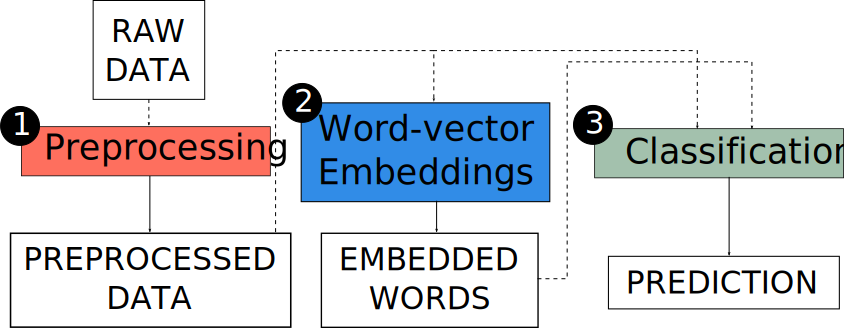
\includegraphics[width=\columnwidth]{graphics/method-steps.pdf} 	
	\caption{Illustration of method steps} 	
	\label{fig:method-steps} 
\end{figure}

\subsection{Preprocessing}\label{sec:method:preprocessing}
The given dataset presents a set of challenges which have to be addressed in order to extract meaningful data. First, the constraint of 140 characters gives rise to a plethora of abbreviations and acronyms. Second, orthography is not observed. We evaluated several methods to address at least some of these issues (as did Bao et al. \cite{bao2014role}).

All these methods aim to reduce the size of our dictionary. They either remove what we considered sentiment-neutral words, or they map differently spelled words onto one. Additionally, inspired by the papers \cite{hemalatha2012preprocessing} and \cite{bao2014role} we implemented the methods \textit{Same-Letter Sequence Removal} and \textit{Negation Connection}.

\subsubsection{Negation Replacement (N)}\label{sec:method:negation-replacement}

Negation replacement substitutes common negated terms with their opposite expressions.

\subsubsection{Word Cancellation (S)}\label{sec:method:word-cancellation}

Word Cancellation removes frequent words that we assumed to be sentiment-free. Examples include: '\textit{i}', '\textit{you}', '\textit{am}'. For the complete list, please contact the authors.

\subsubsection{Tag Removal (R)}\label{sec:method:tag-removal}

Tag removal eliminates the tags \textit{\textless user\textgreater} and \textit{\textless url\textgreater} from every tweet.

\subsubsection{Negation Connection (C) and Negation Disconnection (D)}\label{sec:method:negation-connection}
Negation connection implies that '\textit{n't}' becomes '\textit{nt}', whereas negation disconnection transforms '\textit{n't}' into ' \textit{not}'.

\subsubsection{Short Word Removal (3)}\label{sec:method:short-word-removal}

Short Word Removal removes a word if it consists of two characters or less.

\subsubsection{Same-Letter Sequence Removal (M)}\label{sec:method:same-letter-removal}

If the word contains a letter more than twice in a row, that sequence is shortened down to two characters. For instance, occurrences like '\textit{loool}' are shortened to '\textit{lool}'.

\subsubsection{Word Type Filtering (W)}\label{sec:method:word-type-filtering}

This method categorises every word and then keeps or discards it based on its type. Words were kept if they belonged to one of the types noun, verb, adverb, and adjective.

\subsection{Word embeddings}\label{sec:method:embeddings}

On the basis of preprocessed files, \textit{word-vector embeddings} are produced. Such embedding methods map each word in the vocabulary to a vector in a multi-dimensional space. Semantic relations between words should then be captured by geometric relations between the corresponding vectors, e.g., distance.

In this project, we used and evaluated two well-known embedding methods: \textit{GloVe} \cite{pennington2014glove} and \textit{word2vec} \cite{mikolov2013word2vec}. Coarsely put, both methods work by adapting vectors iteratively such that the dot product of two word vectors is proportional to the probability that the two respective words occur in the same context.

\subsection{Classification}\label{sec:method:classification}

Since a simple and effective approach to learn distributed representations of words was proposed \cite{mikolov2013word2vec}, neural networks advance sentiment analysis substantially.
	
The first such network models, among which are Recursive Neural Network (\cite{socher2011parsing, dong2014adaptive, qian2015learning}), Recursive Neural Tensor Networks (\cite{socher2013reasoning}), and Recurrent Neural Networks (\cite{mikolov2010recurrent}), performed sentiment analysis by utilizing syntax structures of sentences. However, such methods may suffer from syntax parsing errors. In addition, Recurrent Neural Networks (RNN) do not allow information to persist in the long-term. A common solution to this problem was given by LSTM (Long Short-Term Memory) networks, which contain special gates that control the information flow \cite{hochreiter1997long}. 
	
Since LSTM networks are capable of learning long-term dependencies, they are well-suited for natural language modeling. Furthermore, they are less prone to encounter gradient vanishing problems than RNN models. More formally, each cell in LSTM can be computed as follows:

\begin{align}
	X & =\begin{bmatrix}
	h_{t-1} \\
	x_{t} \\
	\end{bmatrix}\\	
	f_{t} & = \sigma(W_{f} \cdot X + b_{f} )  \\
	i_{t} & = \sigma(W_{i} \cdot X + b_{i} )  \\
	o_{t} & = \sigma(W_{o} \cdot X + b_{o} )  \\
	c_{t} & = f_{t} \odot c_{t-1} + i_{t} \odot \mathit{tanh}(W_{c}  \odot X + b_{c})\\
	h_{t} & = o_{t} \odot tanh(c_{t}),
\end{align}		
where $W_{f} , W_{i} , W_{o}, W_{c} \in {\rm I\!R}^{d\times(n + d)}$ are the weighted matrices and $ b_{f},  b_{i}, b_{o}, b_{c} \in {\rm I\!R}^{d}$ are biases to be learned during training, parameterizing the transformations of the input, forget and output gates, respectively. $\sigma$ is the sigmoid function and $\odot$ stands for element-wise multiplication. $ x_{t} \in {\rm I\!R}^{n}$ includes the inputs of LSTM cell unit, representing the word embedding vectors $w_{t}$ (cf. Figure \ref{fig:attention-mechanism}). The vector of hidden layer $t$ is $h_{t} \in {\rm I\!R}^{d}$, where $d$ is the number of hidden units in a cell. Then different approaches can be applied to obtain a vector representation of a sentence. The last hidden vector $h_{N}$ can be considered as the feature representation and also the average of the hidden vectors.

A fully connected hidden layer calculates the transformation $\delta(W_{s} ∗ h_{N} + b_{s})$, where $W_{s} \in {\rm I\!R}^{K,d}$ is the weight matrix, $b_{s} \in {\rm I\!R}^{K}$ the bias, and $\delta$ an  activation function such as the rectified linear unit or $\mathit{tanh}$. The output vector of this layer corresponds to logits that are normalized through a softmax function. Finally, the output returns the probabilities for each class, $y\in \{-1, 1\} $ and $K=2$.
	
A potential issue with this setup is that a neural network needs to be able to compress all the necessary information of a sentence into a fixed-length vector that is fed to the fully connected layer. Inspired by Bahdanau et al. \cite{AttentionBahdanau}, regarding machine translation, we propose to implement an attention mechanism that does not attempt to summarize a whole text into a single vector. Instead, it encodes the input sentence into a sequence of vectors and chooses a subset of these vectors adaptively. Each time that model generates a prediction, it searches for a set of positions in the sentence where the most relevant information is concentrated. Hence, the vector representation is based on the concatenation of the last hidden unit and the context vector computed as weighted sum of all the hidden units. Let $H \in {\rm I\!R}^{d\times N}$ be a matrix consisting of hidden vectors $[h_1, ... , h_N]$ that the LSTM produced, where $z$ is the size of hidden layers for the attention mechanism and $N$ is the length of the given sentence.	
\begin{align}
	M &= \mathit{tanh}(W_h \cdot H)\\
	\alpha &= \mathit{softmax}(w^{T} \cdot M)\\
	r &= H \cdot \alpha^T\\ h^* &= \mathit{tanh}(W_p \cdot  r + W_x \cdot h_N)\\
	y &= \mathit{softmax}(W_s \cdot  h^* + b_s),
\end{align}	
where $W_h \in {\rm I\!R}^{z\times d}, W_p \in {\rm I\!R}^{d\times d},  W_x \in {\rm I\!R}^{d\times d}, w \in {\rm I\!R}^{z}$ are the new matrices of parameters estimated by minimizing the cross-entropy error between $y$ and $\hat{y}$ for all sentences.
	
Luong et al. \cite{luong2015effective} proposed an interesting modification method by categorizing various attention-based models into two broad categories, global and local. The global attention described above computes the scores or alignment ($\alpha$) by taking into account all the hidden states from a sentence. On the other hand, the local attention offers a mechanism that focus on a smaller subsets of words. Compared to the suggested implementation stated in the original paper, we adapted the formulas to perform text classification tasks. In other words, the algorithm selects a window where the alignments decay exponentially around the center. More formally, our model predicts the midpoint of defined interval as follows:  
\begin{align}
	p_t &= N \cdot \mathit{sigmoid}(\upsilon_c \mathit{tanh}(W_c \cdot h_N))\\
	\alpha &= \mathit{softmax}(w^{T} \cdot M) \cdot \exp\bigg(-\frac{(s - p_t)^2}{2\sigma^2}\bigg).
\end{align}
		
$W_c,$  $\upsilon_c$ are the model parameters which will be learned to predict positions. $N$ is the source sentence length. As a result of sigmoid, $p_t \in [0, N]$. To favor alignment points near $p_t$, we place a Gaussian distribution centered around $p_t$. 

The network parameters are learned using Adam optimizer \cite{kingma2014adam}. We set the hyper-parameters to $\eta = 0.001$(learning rate), $\beta_1$ = 0.9, $\beta_2=0.999$ and we linearly decreased $\eta$ whenever the loss function did not improve in the previous 10'000 iterations with a batch size of 64. In Section \ref{sec:results}, we will assess the accuracy of each of those different architectures.

\begin{figure} 	
	\centering 	
	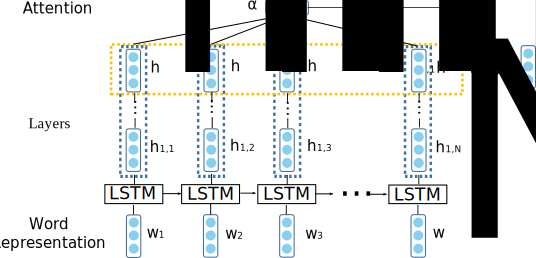
\includegraphics[width=\columnwidth]{graphics/attention-mechanism.pdf} 	
	\caption{Illustration of global attention mechanism} 	
	\label{fig:attention-mechanism} 
\end{figure}

\section{Results}\label{sec:results}

\subsection{Baselines}\label{sec:results:baselines}

We will use the following two algorithms as baselines throughout Section \ref{sec:results}:

\begin{compactitem}
	\item \textbf{\textit{BL1:}} Logistic regression classifier, \textit{GloVe} embeddings produced from the programming assignment script, no preprocessing (Score: 59.92\%)
	\item \textbf{\textit{BL2:}} Logistic regression classifier, \textit{word2vec} embeddings, no preprocessing (Score: 77.21\%)
\end{compactitem}

\subsection{Preprocessing}

\subsubsection{Setup and Process for Evaluation}

We used two classifiers to test the influence of our preprocessing methods. First, we applied a linear classifier that builds on logistic regression (LR). Second, we evaluated our preprocessing method on a recurrent neural network (RNN) (LSTM cells, 1 layer, 150 hidden units, static).

The goal is to improve classification accuracy (fraction of correctly classified tweets over all tweets); this is therefore the metric used to evaluate our preprocessing methods. Each method was evaluated in repeated experiments. We applied each preprocessing method individually and compared the scores to baseline. Next, we ran all combinations of the methods that had improved accuracy.

\subsubsection{Results for Logistic Regression}

\begin{table}
	\centering
	\begin{tabular}{| l | r | r | c}
		\cline{1-3}
		\textbf{Preprocessing method} & \textbf{Score} (\%) & \textbf{Effect} \\ \cline{1-3}
		None (\textit{BL2}) & 77.21 & 0.00 & \\ \cline{1-3}
		3 (Short Word Removal) & 76.65 & -0.56 & \textcolor{red}{$\bm{-}$} \\ \cline{1-3}
		M (Same-Letter Removal) & 77.44 & +0.23 & \textcolor{darkgreen}{$\bm{+}$} \\ \cline{1-3}
		D (Negation Disconnection) & 77.47 & +0.30 & \textcolor{darkgreen}{$\bm{+}$} \\ \cline{1-3}
		C (Negation Connection)	& 77.65 & +0.49 & \textcolor{darkgreen}{$\bm{+}$} \\ \cline{1-3}
		R (Tag Removal)	& 77.80 & +0.64 & \textcolor{darkgreen}{$\bm{+}$}  \\ \cline{1-3}
		N (Negation Replacement) & 77.20 & +0.04 & \textcolor{darkgreen}{$\bm{+}$} \\ \cline{1-3}
		W (Word Type Filtering) & 76.47 & -0.69 & \textcolor{red}{$\bm{-}$} \\ \cline{1-3}
		S (Word Cancellation) & 77.49 & +0.33 & \textcolor{darkgreen}{$\bm{+}$} \\ \cline{1-3}
		MD & 77.61 & +0.44 & \textcolor{darkgreen}{$\bm{+}$}\\ \cline{1-3}
		MR & 77.69 & +0.53& \textcolor{darkgreen}{$\bm{+}$} \\ \cline{1-3}
		DR & 77.77 & +0.60 & \textcolor{darkgreen}{$\bm{+}$}\\ \cline{1-3}
		DS & 77.72 & +0.56 & \textcolor{darkgreen}{$\bm{+}$}\\ \cline{1-3}
		CR & 77.66 & +0.49 & \textcolor{darkgreen}{$\bm{+}$}\\ \cline{1-3}
		RS & 77.77 & +0.61 & \textcolor{darkgreen}{$\bm{+}$}\\ \cline{1-3}
	\end{tabular}
	\caption{Effects of preprocessing methods in the Logistic Regression classifier}
	\label{tab:lr-prep-results-single}
\end{table}

In Table \ref{tab:lr-prep-results-single}, we show the accuracy effect of each method compared to the baseline score \textit{BL2}.

The methods 3 and W reduced accuracy, the other methods improved it, likely because they reduce the number of embeddings and create indicative word associations. The method C worked better than D, congruent with the findings in \cite{bao2014role}. The impact of N is almost negligible, probably because it modifies tweets only marginally. Lastly, R yields a relatively big improvement for the small changes it makes.

%\begin{table}
	\centering
	\begin{tabular}{| l | r | r |}
		\hline
		\textbf{Preprocessing combination} & \textbf{Score} (\%) & \textbf{Effect} \\ \hline
		None & 77.21 & 0.00 \\ \hline
		MD & \cellcolor{green!25}77.61 & \cellcolor{green!25}+0.44 \\ \hline
		MR & \cellcolor{green!25}77.69 & \cellcolor{green!25}+0.53 \\ \hline
		DR & \cellcolor{green!25}77.77 & \cellcolor{green!25}+0.60 \\ \hline
		DS & \cellcolor{green!25}77.72 & \cellcolor{green!25}+0.56 \\ \hline
		CR & \cellcolor{green!25}77.66 & \cellcolor{green!25}+0.49 \\ \hline
		RS & \cellcolor{green!25}77.77 & \cellcolor{green!25}+0.61 \\ \hline		
	\end{tabular}
	\caption{Effects of preprocessing method combinations on accuracy of the Logistic Regression classifier}
	\label{tab:lr-prep-results-comb}
\end{table}

In Table \ref{tab:lr-prep-results-single}, a subset of the results for two preprocessing methods are shown. For the full results, please refer to the appendix.

Note that the pairs involving R improved accuracy the most. However, it is unclear to us why these combinations lead to worse accuracy compared to R alone, especially since the combined preprocessing methods do not interfere with each other. Contrary to pairs involving R, the remaining combinations improved nearly by the sum of their single-scores. We assign this effect, again, to the reduced word embeddings and strengthening of common word associations.

\subsubsection{Results for RNN}

Table \ref{tab:rnn-prep-results-single} contains information on how the classification accuracy of a Recurrent Neutral Network (RNN) is influenced by our preprocessing methods. One quickly notices that, unlike in the case of a logistic regression, preprocessing the tweets leads to a decrease in accuracy in more cases.

\begin{table}
	\centering
	\begin{tabular}{| l | r | r | c}
		\cline{1-3}
		\textbf{Preprocessing method} & \textbf{Score} (\%) & \textbf{Effect} & \\ \cline{1-3}
		None & 81.24 & 0.00  & \\ \cline{1-3}
		3 (Short Word Removal) & 80.45 & -0.79 & \textcolor{red}{$\bm{-}$}\\ \cline{1-3}
		M (Same-Letter Removal) & 81.89 & +0.64 & \textcolor{darkgreen}{$\bm{+}$}\\ \cline{1-3}
		D (Negation Disconnection) & 81.05 & -0.20 & \textcolor{red}{$\bm{-}$} \\ \cline{1-3}
		C (Negation Connection)	& 81.28 & +0.03  & \textcolor{darkgreen}{$\bm{+}$}\\ \cline{1-3}
		R (Tag Removal)	& 80.90 & -0.34 &  \textcolor{red}{$\bm{-}$} \\ \cline{1-3}
		N (Negation Replacement) & 80.94 & -0.30 & \textcolor{red}{$\bm{-}$} \\ \cline{1-3}
		W (Word Type Filtering) & 80.98 & -0.26 & \textcolor{red}{$\bm{-}$} \\ \cline{1-3}
		S (Word Cancellation)	& 81.72 & +0.47  & \textcolor{darkgreen}{$\bm{+}$}\\ \cline{1-3}
		MC & 81.30 & +0.06  & \textcolor{darkgreen}{$\bm{+}$}\\ \cline{1-3}
		MS & 81.96 & +0.71  & \textcolor{darkgreen}{$\bm{+}$}\\ \cline{1-3}
		CS & 81.96 & +0.71  & \textcolor{darkgreen}{$\bm{+}$}\\ \cline{1-3}
		MCS & 81.92 & +0.68  & \textcolor{darkgreen}{$\bm{+}$}\\ \cline{1-3}
	\end{tabular}
	\caption{Effects of preprocessing methods in the RNN classifier}
	\label{tab:rnn-prep-results-single}
\end{table}
%\begin{table}
	\centering
	\begin{tabular}{| l | r | r |}
		\hline
		\textbf{Preprocessing combination} & \textbf{Score} (\%) & \textbf{Effect} \\ \hline
		None & 81.24 & 0.00 \\ \hline
		MC & \cellcolor{green!25}81.30 & \cellcolor{green!25}+0.06 \\ \hline
		MS & \cellcolor{green!25}81.96 & \cellcolor{green!25}+0.71 \\ \hline
		CS & \cellcolor{green!25}81.96 & \cellcolor{green!25}+0.71 \\ \hline
		MCS & \cellcolor{green!25}81.92 & \cellcolor{green!25}+0.68 \\ \hline	
	\end{tabular}
	\caption{Effects of preprocessing method combinations on accuracy of the Logistic Regression classifier}
	\label{tab:rnn-prep-results-comb}
\end{table}

We notice that word cancellation is not necessarily a source of inaccuracy, since both improving as well as damaging methods (S and 3) perform some kind of word cancellation. Accuracy effects may thus depend on \textit{which} words are removed.

Unexpectedly, the gains achievable when using method M alone are virtually neutralized when using it in combination with method C. Surprising on this note is that method C significantly helps method S.

\subsubsection{Comparison of Classifiers}

Our results show that the effect of a preprocessing method is heavily dependent on the used classifier. The following examples illustrate this finding:
\begin{compactitem}
	\item Negation replacement (N) greatly affects RNN whereas LR barely notices it.
	\item Negation connection (C) greatly helped LR but is negligible for RNN.
	\item Tag removal (R) has a positive effect on LR accuracy but a negative effect on RNN accuracy.
\end{compactitem}

In conclusion, handling same-letter sequences is a safe improvement, given that both LR and RNN seem to benefit from it. They also agreed on negation connection, although care should be taken when combining it with other preprocessing method. Lastly, our method to remove simple, common words also helps either model.

\subsection{Word-Vector Embeddings}
\begin{table}
	\centering
	\begin{tabular}{| l | l | l | r |}
		\hline
		\textbf{Embedding} & \textbf{Classifier} & \textbf{Preprocessing} & \textbf{Score} (\%) \\ \hline
		\multirow{4}{*}{GloVe} & \multirow{2}{*}{LR} & None & 67.82 \\ \cline{3-4}
		& & M & 68.42 \\ \cline{2-4}
		& \multirow{2}{*}{RNN} & None & 75.36 \\ \cline{3-4}
		& & M & 75.81 \\ \hline
		\multirow{4}{*}{word2vec} & \multirow{2}{*}{LR} & None & 77.21 \\ \cline{3-4}
		& & M & 77.44 \\ \cline{2-4}
		& \multirow{2}{*}{RNN} & None & 81.24 \\ \cline{3-4}
		& & M & 81.89 \\ \hline
	\end{tabular}
	\caption{Effects of performance on classification accuracy}
	\label{tab:embedding-evaluation}
\end{table}
We evaluated the effects of the different embedding methods from Section \ref{sec:method:embeddings} on classification accuracy. In these experiments, the results in Table \ref{tab:embedding-evaluation} were obtained: Clearly, \textit{word2vec} performs considerably better than \textit{GloVe}, independently of classifier and preprocessing used.
\subsection{Classification}
\begin{table*}
	\centering
	\begin{tabular}{|l  r  r  l  r|}
		\hline
		\textbf{Classifier} & \textbf{Units} & \textbf{Layers} & \textbf{Embeddings} & \textbf{Score} (\%) \\ \hline
		Logistic Regression (\textit{BL1}) & - & - & GloVe & 59.92 \\ \hline
		Logistic Regression (\textit{BL2}) & - & - & word2vec  & 77.21 \\ \hline
		LSTM & 252 & 1 & word2vec & 87.22 \\ \hline
		LSTM & 252 & 2 & word2vec & 87.38 \\ \hline
		LSTM + Global Attention &  200 & 2 & word2vec & 87.52 \\ \hline
		LSTM + Local Attention &  200 & 2 & word2vec & 87.56 \\ \hline				
		LSTM & 190 & 3 & word2vec & 87.20 \\ \hline
		LSTM + Global Attention & 190 & 3 & word2vec &  87.74 \\ \hline
		LSTM + Local Attention &  190  & 3 & word2vec & 87.28 \\ \hline
		LSTM & 150 & 4 & word2vec & 87.96 \\ \hline		
		LSTM + Global Attention & 150 & 4 & word2vec & 87.72 \\ \hline
		LSTM + Local Attention & 150 & 4 & word2vec & 87.67 \\ \hline		
	\end{tabular}
	\caption{Accuracy results of RNN classifier}
	\label{tab:rnn-class-results}
\end{table*}
Selected results of classification are displayed in Table \ref{tab:rnn-class-results}. All classification evaluation experiments were performed using a skipgram model of window size 5 and filtering words that occur less than 5 times with an embedding dimension of 100, a dropout of 0.75, and a vocabulary size of 89'000 on the test set.

It is enlightening to analyze which model more accurately predicts the sentiment given the results obtained on the test set in the ranking system (Kaggle). In our study, we observe that in general, precision is increased by inserting more layers and keeping approximately the same number of parameters in our classifiers. Notwithstanding, the marginal benefit from incrementing the number of layers clearly diminishes. Secondly, adding an attention mechanism sightly boots the accuracy. However this pattern is no longer observable when using four layers. Surprisingly, the local attention does not obtain a better score than the global one. 

\section{Discussion}

Judging from the results in the previous section, our step-wise optimization approach yielded counter-intuitive findings as well as notable improvements in accuracy.

We want to highlight two unexpected findings and give possible explanations for them:

First, we wrongly assumed that most words removed by preprocessing methods 3 and W are neutral regarding sentiment and thus not helpful in classification. Possibly, removing many words could have the effect that context windows become more diverse. If co-occurrence counts are smaller, vector embeddings  become more imprecise, which would explain the drop in classification accuracy.  

Second, the benefit of preprocessing methods is heavily dependent on the used classifier. Source of these differences could be the categorically different \textit{modus operandi} of the two classifiers: Whereas LR condenses all vectors relating to tweet words into a single vector, RNN processes individual word vectors in the word order of the tweet. Structure may render even insignificant words more relevant. For example, prepositions are not very meaningful on their own but become more meaningful when incorporated in a sentence structure.

On the contrary, the benefit of single embedding methods is very unambiguous. Not only did \textit{word2vec} embeddings lead to better results, but their production was also far faster. However, this observation can be partially explained by the fact that we used the C code to produce $word2vec$ embeddings and Python code to produce $GloVe$ embeddings.


\section{Summary}
We described our deep learning approach to Twitter sentiment analysis on phrase level. We gave a detailed description of our 3-step process consisting of preprocessing, word-vector embeddings production, and classification. In each step, we evaluated several different approaches and combined the best-performing solutions from every step. The resulting model demonstrates state-of-the-art performance and provides a novel approach by introducing an attention mechanism to our multi-layer LSTM model. 

\pagebreak
\bibliography{project-report}

\end{document}
